\documentclass{article}

\title{CS3031 - Project 1}
\author{Paolo Moloney - 16325409}

\usepackage{listings}
\usepackage{color}
\usepackage{setspace}
\usepackage{graphicx}

\definecolor{Code}{rgb}{0,0,0}
\definecolor{Decorators}{rgb}{0.5,0.5,0.5}
\definecolor{Numbers}{rgb}{0.5,0,0}
\definecolor{MatchingBrackets}{rgb}{0.25,0.5,0.5}
\definecolor{Keywords}{rgb}{0,0,1}
\definecolor{self}{rgb}{0,0,0}
\definecolor{Strings}{rgb}{0,0.63,0}
\definecolor{Comments}{rgb}{0,0.63,1}
\definecolor{Backquotes}{rgb}{0,0,0}
\definecolor{Classname}{rgb}{0,0,0}
\definecolor{FunctionName}{rgb}{0,0,0}
\definecolor{Operators}{rgb}{0,0,0}
\definecolor{Background}{rgb}{0.98,0.98,0.98}

\lstdefinelanguage{Python}{
	numbers=left,
	numberstyle=\footnotesize,
	numbersep=1em,
	xleftmargin=1em,
	framextopmargin=2em,
	framexbottommargin=2em,
	showspaces=false,
	showtabs=false,
	showstringspaces=false,
	frame=l,
	tabsize=4,
	% Basic
	basicstyle=\ttfamily\small\setstretch{1},
	backgroundcolor=\color{Background},
	% Comments
	commentstyle=\color{Comments}\slshape,
	% Strings
	stringstyle=\color{Strings},
	morecomment=[s][\color{Strings}]{"""}{"""},
	morecomment=[s][\color{Strings}]{'''}{'''},
	% keywords
	morekeywords={import,from,class,def,for,while,if,is,in,elif,else,not,and,or,print,break,continue,return,True,False,None,access,as,,del,except,exec,finally,global,import,lambda,pass,print,raise,try,assert},
	keywordstyle={\color{Keywords}\bfseries},
	% additional keywords
	morekeywords={[2]@invariant,pylab,numpy,np,scipy},
	keywordstyle={[2]\color{Decorators}\slshape},
	emph={self},
	emphstyle={\color{self}\slshape},
	%
}

\begin{document}

\maketitle
\newpage

\tableofcontents
\newpage

\section{Specification}

The objective of this project is to implement a proxy server with the following features:

\begin{enumerate}
	\item Respond to HTTP and HTTPS requests, displaying them and the responses on a management console.
	\item Handle websocket connections.
	\item Block selected URLs via the console.
	\item Cache requests locally to save bandwidth.
	\item Handle multiple requests simultaneously.
\end{enumerate}

\newpage

\section{Implementation}

I chose to implement the proxy server in Python 3, using the following modules:

\begin{enumerate}
	\item \texttt{socket}: provides low-level access to the BSD socket interface
	\item \texttt{threading}: provides higher-level threading interfaces based on the low-level \texttt{\_thread} module
\end{enumerate}

The following diagram outlines the design decisions I made.

\begin{figure}[h]
	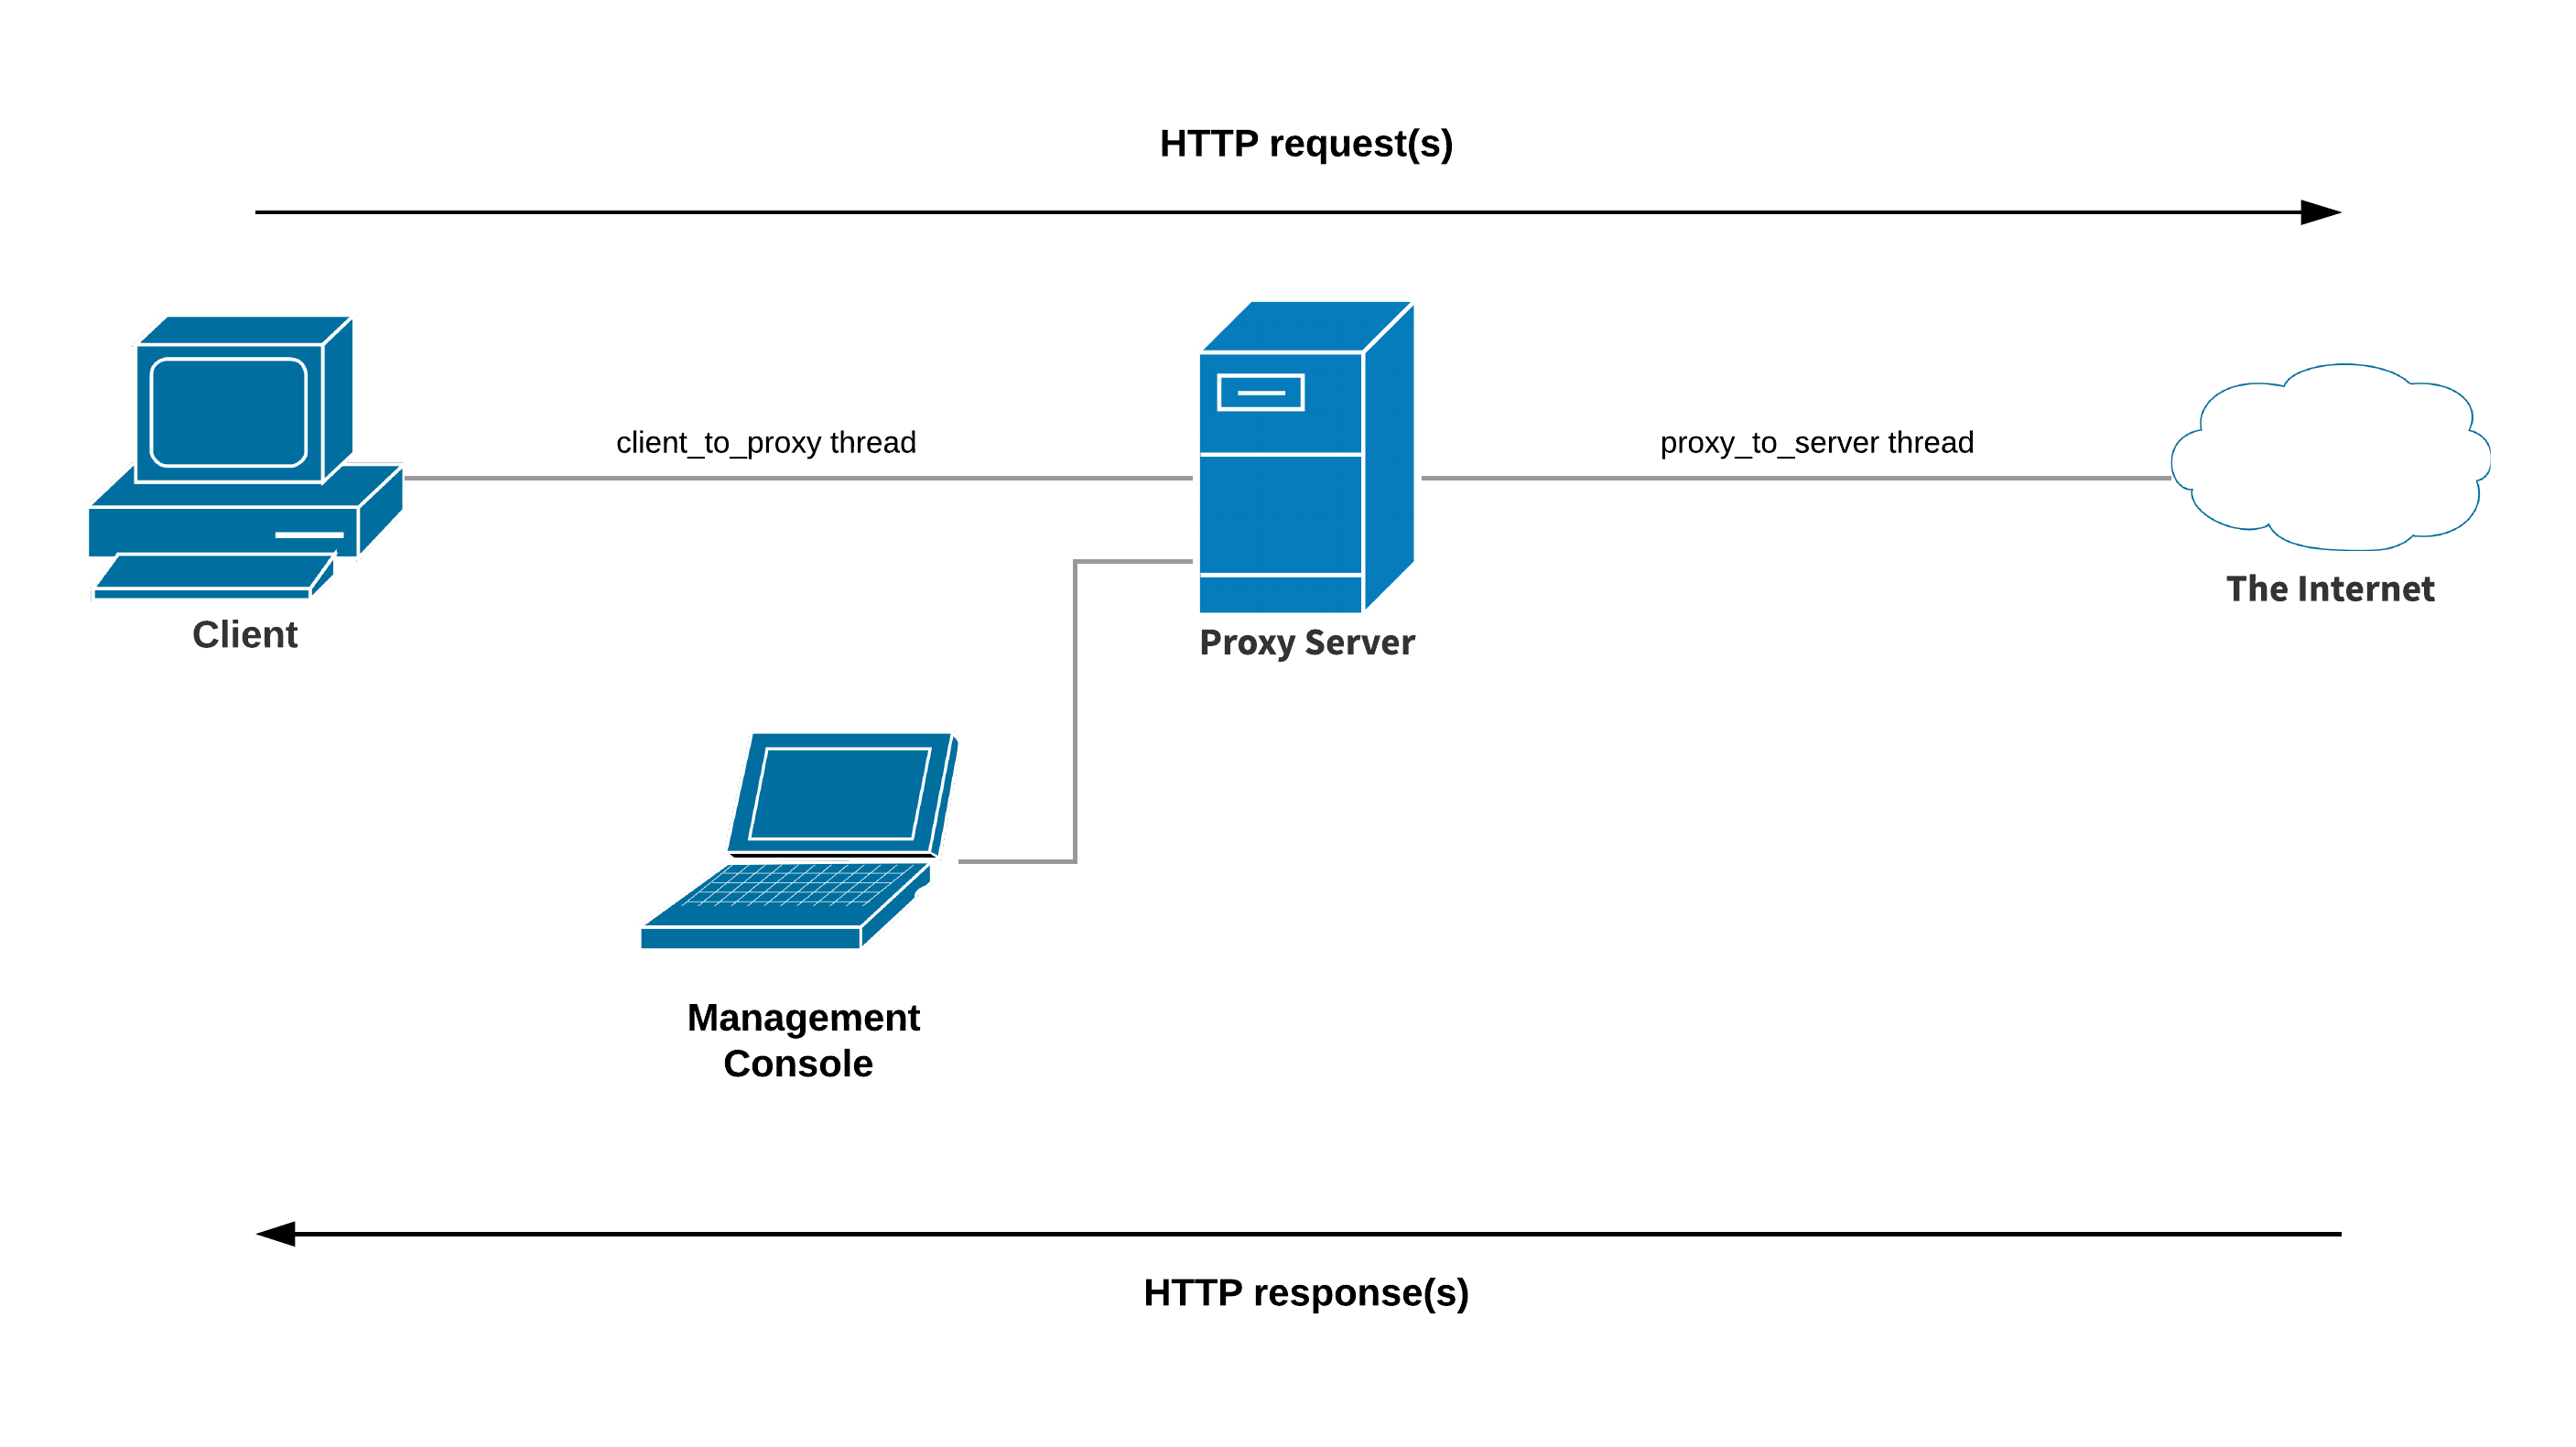
\includegraphics[width=\linewidth]{proxy_diagram.png}
	\caption{Proxy server diagram}
	\label{fig:diagram}
\end{figure}

\newpage

\section{Code}
\lstinputlisting[language=Python]{../proxy.py}
\end{document}
